\documentclass[a4paper, 12pt]{report}
\usepackage[spanish]{babel}
\usepackage[utf8]{inputenc}
\usepackage{textcomp}
\usepackage{booktabs}
\usepackage{amssymb}
\usepackage{bussproofs}
\usepackage{fancyhdr}
\usepackage{graphicx}
\usepackage{amsmath}

\usepackage{hyperref}
\hypersetup{
    colorlinks=true,
    linkcolor=blue,
    filecolor=magenta,
    urlcolor=cyan,
}

\pagestyle{fancy}
\lhead{Almeida, Figueroa \& Ibarra}
\chead{Tarea 1}
\rhead{\today}

\begin{document}
\begin{titlepage}
    \centering
    {\scshape\Huge Universidad Nacional Autónoma de México \par}
    \vspace{1.25cm}
    {\scshape\huge Fundamentos de Bases de Datos\par}
    \vspace{1.25cm}
    {\huge\bfseries Tarea 1\par}
    \vspace{1.25cm}
    {\Large\textsc Almeida Rodríguez Jerónimo\par}
    \vspace{.1cm}
    {\large\texttt{jalrod@ciencias.unam.mx}\par}
    \vspace{0.25cm}
    {\Large\textsc Figueroa Sandoval Gerardo Emiliano\par}
    \vspace{.1cm}
    {\large\texttt{efs\_070@ciencias.unam.mx}\par}
    \vspace{0.25cm}
    {\Large\textsc Ibarra Moreno Gisselle \par}
    \vspace{.1cm}
    {\large\texttt{gisselleib@ciencias.unam.mx}\par}
    \vspace{1.5cm}
    \vfill
    \begin{figure}[hb!]
        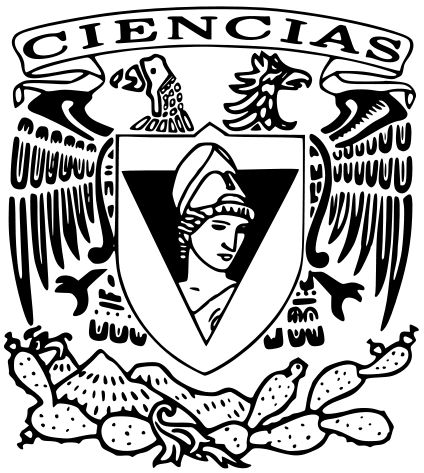
\includegraphics[width=.3\textwidth]
            {../logos/escudo_f-ciencias.png}\hfill
        
\includegraphics[width=.3\textwidth]
            {../logos/Escudo_UNAM.png}\hfill
    \end{figure}
\end{titlepage}
\begin{enumerate}
\item[1)]{
\begin{enumerate}
    \item[a)]{¿Por qué elegirías almacenar datos en un sistema de base
	 de datos en lugar de simplemente almacenarlos utilizando el
	 sistema de archivos de un sistema operativo? ¿En qué casos no
	 tendría sentido utilizar un sistema de base de datos?\\

	 No podría guardar cantidades grandes de información, el acceso
	 y las busquedas de información grandes	toman demasiado tiempo
	 en un sistema de archivos.Tampoco se pueden ordenar y actualizar
	 constantemente, tampoco podría modificar el esquema de la base
	 de datos sin tener que modificar completamente los archivos.\\
	 El sistema de archivos no es seguro incluso con un sistema
	 de contraseñas ya que no podemos asegurar la integridad de los
	 datos. No es dinámico, para que más personas tuvieran acceso a
	 mi base de datos tendría que pasarles los datos manualmente, lo cual es muy ineficiente.\\
	 No tendría sentido usar una base de datos cuando se tienen muy
	 pocos datos a guardar.}
    \item[b)]{¿Qué ventajas y desventajas encuentras al trabajar con una
	 base de datos?\\
	 \textbf{Ventajas:}
	 \begin{itemize}
	 	\item Se pueden sincronizar datos en ella
	 	\item Se puede modificar la estructura fácilmente
	 	\item Garantizan la fiabilidad
	 	\item Existen por un periodo largo de tiempo
	 	\item Permite controlar la redundancia
	 	\item Son independientes a los programas que proporcionan las
	 	vistas.
	 \end{itemize}
 	 \textbf{Desventajas:}
 	 \begin{itemize}
 	 	\item Son costosas.
 	 	\item No cualquiera puede manejarla, se necesita alguien
 	 	especializado.
 	 	\item Se requiere de capacitación para su manejo.
 	 \end{itemize} }%Pregunta E.%
    \item[c)]{Investiga cuáles serían las responsabilidades de un DBA y las de
                un diseñador de bases de datos.\\
        Entre las responsabilidades de un administrador de bases de datos se
        encuentran la instalación y actualización de las herramientas de administración,
        el desarrollo de respaldos y pruebas para recuperar la información de la BD,
        saber modificar el esquema de la BD, velar por su integridad, garantizar
        acceso continuo todo el tiempo que sea posible y el mejor desempeño de la BD
        entre otras cosas tipo mantenimiento y así.\cite{DBA}\\
        Por su parte, un diseñador de bases de datos se encarga de determinar qué
        información va a ser almacenada y cómo se relacionan los datos entre ellos.
        Finalmente, se estructuran los datos logicamente. }
    \item[d)]{Investiga  cuáles  serían  los distintos tipos de
     usuarios finales de una base de datos, indica las principales
     actividades que realizaría cada uno de ellos. \\\\
     \textbf{Usuarios Finales.} Acceden a la base de datos desde
     alguna terminal, pueden utilizar un lenguaje de consultar o un
     programa de aplicación. Tenemos distintos tipos de usuarios
     finales:
     \begin{itemize}
       \item \textbf{Esporádicos.} Acceden de vez en cuando, no
       siempre requieren la misma información. Utilizan lenguajes
       sofisticados de consulta para especificar su solicitud.\\
       \item \textbf{Paramétricos.} Estos usuarios hacen consultas
       y actualizan la base de datos constantemente, no necesitan
       aprender del lenguaje de consultas, ya que normalmente
       utilizan una interfaz gráfica diseñada para ese propósito.
       \item \textbf{Sofisticados o avanzados.} Son profesionales,
       tales como ingenieros, científicos y otros que están muy
       familiarizados con el sistemas manejador de bases de datos.
       Estos usuarios suelen hacer uso de sus conocimientos para
       satisfacer requerimientos complejos.
       \item \textbf{Autónomos.} Mantienen sus propias bases de datos, utilizando paquetes de programas que facilitan su uso.

     \end{itemize}}
    \item[e)]{Explica las diferencias entre la independencia de datos física y lógica. ¿Cuál es más difícil de lograr y por qué?  }%Pregunta E.%
    \item[f)]{}
    \item[g)]{Indica las principales características de los modelos de
    datos más representativos. ¿Cuáles serían las diferencias
    entre los  modelos relacional, orientado a objetos,
    semiestructurado y objeto –relacional?\\
    \textbf{Modelo Relacional.}Los datos se perciben como tablas,
    es un sistema cerrado, todas las operaciones son siempre tablas.\\
    \textbf{Modelo Orientado a Objetos.} Los datos se modelan como
    objetos, se tiene comportamiento (métodos o funciones) y estado.\\
    \textbf{Modelo Semiestructurado.} Es una colección de nodos y
    cada nodo tiene datos con diferentes esquemas, esto lo hace un
    sistema menos rígido.\\
    \textbf{Modelo Objeto-Relacional} Representa los datos como tablas,
    permite construir tipos de objetos complejos, capacidad para
    encapsular y asociar métodos a los objetos.}
    \item[h)]{Elabora una línea de tiempo, en dónde indiques los principales hitos en el desarrollo de las BDs.}%Pregunta E.%
    \item[i)]{}
    \item[j)]{Supón  que  un banco pequeño desea  almacenar  su
    información  en una  base  de  datos  y  le gustaría comprar
    el SMBD que  tenga  la  menor  cantidad  de  características
    posibles. Está interesado en ejecutar la aplicación en una sola computadora personal y no se planea compartir la
    información  con  nadie.  Para  cada  una  de  las
    siguientes  características  explica  por  qué  se debería o
    no incluir en el SMBD que se desea comprar (suponiendo que se
    pueden comprar por separado): \textbf{seguridad, control de
    concurrencia, recuperación en caso de fallas, lenguaje de
    consulta, mecanismo de vistas, manejo de transacciones}\\
    \textbf{Seguridad:} Es necesario comprarlo, ya que no quieren
    compartir la información con nadie, por lo tanto los datos
    se deben proteger y evitar que cualquiera pueda acceder a
    ellos.\\
    \textbf{Control de concurrencia:} No se necesita incluir ya que
    se planea ejecutar la aplicación en una sola computadora
    personal, por lo que el control de concurrencia sería
    completamente innecesario si no va a ser utilizados por varias
    personas a la vez.\\
    \textbf{Recuperación en caso de fallas:} Es necesario, ya que
    la aplicación solo funcionará en una sola computadora personal,
    por lo que si hubiera algún tipo de falla, toda la información
    se perdería y no habría ningún otro lugar para recuperarlo.\\
    \textbf{Lenguaje de consulta:} Es necesario, para poder acceder,
    actualizar y guardar los datos en la base de datos.\\
    \textbf{Mecanismo de vista}\\
    \textbf{Manejo de transacciones}No es necesario\\}
\end{enumerate}
}
\item[2)]{
\begin{enumerate}
    \item[a)]{}
    \item[b)]{¿Qué son las bases de datos NoSQL? indica el modelo de datos utilizado y algunos proveedores. }%Pregunta E.%
    \item[c)]{}
\end{enumerate}
}
\end{enumerate}
\begin{thebibliography}{3}
    \bibitem[DBA]{DBA}
        Wikipedia. (2019).\\
        Administrador de Banco de Dados.\\
        Visitado el 22 de agosto del 2019.\\
        \url{https://pt.wikipedia.org/wiki/Administrador_de_banco_de_dados}
    \bibitem[DBD]{DBD}
        Wikipedia. (2019).\\
        Database design.\\
        Visitado el 23 de agosto del 2019.\\
        \url{https://en.wikipedia.org/wiki/Database_design}
\end{thebibliography}
\end{document}
